\documentclass[a4paper,11pt]{book}
%\documentclass[a4paper,twoside,11pt,titlepage]{book}
\usepackage[pdfborder={000}, hidelinks]{hyperref} %referencia
\usepackage{listings}
\usepackage[utf8]{inputenc}
\usepackage[spanish, es-tabla]{babel}
\usepackage{eurosym}
\usepackage{csvsimple}
%\usepackage{cite}

\usepackage[loadshadowlibrary]{todonotes}
\usepackage{float, subcaption}
\usepackage{amsmath}
\usepackage{colortbl}
\usepackage{multirow}
\usepackage{multicol}
\definecolor{M1}{RGB}{255,199,2}
\usepackage{algorithm}% http://ctan.org/pkg/algorithms
\usepackage{algpseudocode}
\usepackage{rotating}
\usepackage{amsmath}
\usepackage{dirtytalk}
\usepackage{xcolor}
\usepackage{tikz}
\usepackage{makecell}

\newcommand{\code}{\lstinline}
\usepackage{dirtree}

\usepackage{csquotes}
\usepackage{microtype}
\usepackage[backend=biber, defernumbers=true, citestyle=numeric-comp, bibstyle=ieee, sorting=none]{biblatex}

\DeclareBibliographyCategory{cited}
\AtEveryCitekey{\addtocategory{cited}{\thefield{entrykey}}}
% Configurando BibLaTeX
\DefineBibliographyStrings{spanish}{
  url = {URL},
  andothers={et ~al\adddot}
}

\addbibresource{bibliografia/bibliografia.bib}

\setlength{\parindent}{0pt}

\definecolor{ugr_yellow}{rgb}{1.0, 0.78, 0}

%\usepackage[style=list, number=none]{glossary} %
%\usepackage{titlesec}
%\usepackage{pailatino}
\newcommand{\norm}[1]{\lVert#1\rVert_2}

\decimalpoint
\usepackage{dcolumn}
\newcolumntype{.}{D{.}{\esperiod}{-1}}
\makeatletter
\addto\shorthandsspanish{\let\esperiod\es@period@code}
\makeatother


%\usepackage[chapter]{algorithm}
\RequirePackage{verbatim}
%\RequirePackage[Glenn]{fncychap}
\usepackage{fancyhdr}
\usepackage{graphicx}
\usepackage{afterpage}

\usepackage{longtable}

% ********************************************************************
% Re-usable information
% ********************************************************************
\newcommand{\myTitle}{Estudio y Análisis de Metaheurísticas Modernas para el problema de la Selección de Características\xspace}
\newcommand{\myDegree}{Grado en Ingeniería Informática\xspace}
\newcommand{\myName}{Miguel García López\xspace}
\newcommand{\myProf}{Daniel Molina Cabrera\xspace}
%\newcommand{\mySupervisor}{Put name here\xspace}
\newcommand{\myFaculty}{Escuela Técnica Superior de Ingenierías Informática y de
Telecomunicación\xspace}
\newcommand{\myFacultyShort}{E.T.S. de Ingenierías Informática y de
Telecomunicación\xspace}
\newcommand{\myDepartment}{Departamento de Ciencias de la Computación e Inteligencia Artificial \xspace}
\newcommand{\myUni}{\protect{Universidad de Granada}\xspace}
\newcommand{\myLocation}{Granada\xspace}
\newcommand{\myTime}{\today\xspace}
\newcommand{\myVersion}{Version 0.1\xspace}


\hypersetup{
pdfauthor = {\myName (email (en) ugr (punto) es)},
pdftitle = {\myTitle},
pdfsubject = {},
pdfkeywords = {palabra_clave1, palabra_clave2, palabra_clave3, ...},
pdfcreator = {LaTeX con el paquete ....},
pdfproducer = {pdflatex}
}
%\hyphenation{}


%\usepackage{doxygen/doxygen}
%\usepackage{pdfpages}
\usepackage{url}
\usepackage{colortbl,longtable}
\usepackage[stable]{footmisc}
%\usepackage{index}
\usepackage{booktabs} % Required for \bottomrule
\usepackage{adjustbox}
\usepackage{pdflscape}
\usepackage{changepage}

%\makeindex
%\usepackage[style=long, cols=2,border=plain,toc=true,number=none]{glossary}
%\makeglossary

% Definición de comandos que me son tiles:
%\renewcommand{\indexname}{Índice alfabético}
%\renewcommand{\glossaryname}{Glosario}

\pagestyle{fancy}
\fancyhf{}
\fancyhead[LO]{\leftmark}
\fancyhead[RE]{\rightmark}
\fancyhead[RO,LE]{\textbf{\thepage}}
\renewcommand{\chaptermark}[1]{\markboth{\textbf{#1}}{}}
\renewcommand{\sectionmark}[1]{\markright{\textbf{\thesection. #1}}}

\setlength{\headheight}{1.5\headheight}

\newcommand{\HRule}{\rule{\linewidth}{0.5mm}}
%Definimos los tipos teorema, ejemplo y definición podremos usar estos tipos
%simplemente poniendo \begin{teorema} \end{teorema} ...
\newtheorem{teorema}{Teorema}[chapter]
\newtheorem{ejemplo}{Ejemplo}[chapter]
\newtheorem{definicion}{Definición}[chapter]

\definecolor{gray97}{gray}{.97}
\definecolor{gray75}{gray}{.75}
\definecolor{gray45}{gray}{.45}
\definecolor{gray30}{gray}{.94}

\lstset{ frame=Ltb,
     framerule=0.5pt,
     aboveskip=0.5cm,
     framextopmargin=3pt,
     framexbottommargin=3pt,
     framexleftmargin=0.1cm,
     framesep=0pt,
     rulesep=.4pt,
     backgroundcolor=\color{gray97},
     rulesepcolor=\color{black},
     %
     stringstyle=\ttfamily,
     showstringspaces = false,
     basicstyle=\normalsize\ttfamily,
     commentstyle=\color{gray45},
     keywordstyle=\bfseries,
     %
     numbers=left,
     numbersep=6pt,
     numberstyle=\tiny,
     numberfirstline = false,
     breaklines=true,
   }
 
% minimizar fragmentado de listados
\lstnewenvironment{listing}[1][]
   {\lstset{#1}\pagebreak[0]}{\pagebreak[0]}

\lstdefinestyle{CodigoC}
   {
	basicstyle=\scriptsize,
	frame=single,
	language=C,
	numbers=left
   }
\lstdefinestyle{CodigoC++}
   {
	basicstyle=\small,
	frame=single,
	backgroundcolor=\color{gray30},
	language=C++,
	numbers=left
   }

 
\lstdefinestyle{Consola}
   {basicstyle=\scriptsize\bf\ttfamily,
    backgroundcolor=\color{gray30},
    frame=single,
    numbers=none
   }


\newcommand{\bigrule}{\titlerule[0.5mm]}


%Para conseguir que en las páginas en blanco no ponga cabecerass
\makeatletter
\def\clearpage{%
  \ifvmode
    \ifnum \@dbltopnum =\m@ne
      \ifdim \pagetotal <\topskip
        \hbox{}
      \fi
    \fi
  \fi
  \newpage
  \thispagestyle{empty}
  \write\m@ne{}
  \vbox{}
  \penalty -\@Mi
}
\makeatother

\usepackage{pdfpages}

% % Temporarly
% \usepackage{fancyhdr}
% \pagestyle{fancyplain}
% \fancyhead{}
% \lfoot{\scriptsize\LaTeX}
% \cfoot{\hyperlink{listoftodos}{ToDoList} || \hyperlink{tableofcontents}{TableOfContents}}
% \rfoot{\small\thepage}

\begin{document}
\begin{titlepage}
 
 
\newlength{\centeroffset}
\setlength{\centeroffset}{-0.5\oddsidemargin}
\addtolength{\centeroffset}{0.5\evensidemargin}
\thispagestyle{empty}

\noindent\hspace*{\centeroffset}\begin{minipage}{\textwidth}

\centering

\includegraphics[width=0.9\textwidth]{imagenes/UGR-MARCA-02-color.png}\\[1.4cm]

\textsc{ \Large TRABAJO FIN DE GRADO\\[0.2cm]}
\textsc{ INGENIERÍA INFORMÁTICA}\\[1cm]
% Upper part of the page
% 
% Title
{\Huge\bfseries Estudio y Análisis de Metaheurísticas modernas para el problema de Selección de Características\\
}
\noindent\rule[-1ex]{\textwidth}{3pt}\\[3.5ex]
\end{minipage}

\vspace{1.4cm}
\noindent\hspace*{\centeroffset}\begin{minipage}{\textwidth}
\centering

\textbf{Autor}\\ {Miguel García López}\\[2.5ex]
\textbf{Directores}\\
{Daniel Molina Cabrera}\\[2cm]

\includegraphics[width=0.3\textwidth]{imagenes/etsiit_logo.png}\\[0.1cm]
\textsc{Escuela Técnica Superior de Ingenierías Informática y de Telecomunicación}\\
\textsc{---}\\
Granada, Enero de 2024
\end{minipage}
%\addtolength{\textwidth}{\centeroffset}
%\vspace{\stretch{2}}
\end{titlepage}


\begin{frame}[plain]
  
  \titlepage

  
  \begin{tikzpicture}[overlay,remember picture]
      \node[left=-0.30cm] at (current page.0){
          
\includegraphics[scale=0.142]{imagenes/IntroBackground}
      };
  \end{tikzpicture}
\end{frame}

\note{
Mi nombre es Miguel García López, estudiante del Grado de Ingeniería Informática. Hoy presento mi proyecto de TFG, gracias a la tutorización del profesor Daniel Molina Cabrera. En esta presentación, se explicará el problema de selección de características y la aplicación de metaheurísticas al mismo. Se realizará un estudio y análisis de varias versiones y varios algoritmos.
}

\begin{frame}[noframenumbering]
    \frametitle{Índice}
  \begin{multicols}{2}
  \tableofcontents
  \end{multicols}
\end{frame}


\frontmatter
\mainmatter

\tableofcontents
\listoffigures
\listoftables
\setlength{\parskip}{5pt}

\chapter{Introducción}
\section{Definición del problema}
El problema de la selección de características se define como el proceso de
seleccionar un subconjunto de características relevantes~\cite{miao_survey_2016}. Una característica es
una propiedad individual medible de un fenómeno concreto. Este problema es
considerado un problema \textbf{NP duro}. La reducción de dimensionalidad, y con
ello de características, suele ser necesario a la hora de crear un modelo predictivo por medio
del aprendizaje automático ya que muchas de las características
dentro de un conjunto de datos pueden no llegar a ser relevantes para solucionar
aquellos problemas que se intentan solucionar, ya sea por que no aporta información,
porque puede ser agrupada junto a otras tantas en una sola propiedad o incluso porque hay ruido
en los datos, lo cual es inevitable~\cite{Mostafa2012}.\\[6pt]
Gracias a la reducción de características es posible mejorar tanto la capacidad de generalización
como la precisión del modelo predictivo gracias a la reducción de \textit{ruido}.\\[6pt]
Siendo $f$ la función objetivo a predecir, $H^n$ el conjunto de hipótesis o conjunto de modelos
de dimensión $n$ posibles, $h^*(x)$ el mejor modelo aprendido y $x$ una variable de entrada. El ruido conocido
como ruido estocástico es aquel que atiende a una variación aleatoria que
puede surgir de diversos factores, como mediciones imprecisas de señales o la falta de
precisión en sensores. Por otro lado, el ruido determinista está directamente
relacionado con la complejidad de un modelo. Su presencia aumenta la probabilidad de
sobreajuste. El ruido determinista puede explicarse como la parte de la función $f$ que el conjunto
de hipótesis $H^n$ no puede capturar, es decir, $f(x) - h^*(x)$. Este tipo de ruido se
considera así porque la función (modelo) no es lo suficientemente compleja como para comprender
esa parte. Este ruido depende de $H^n$ y permanece constante para un valor dado de $x$~\cite{Mostafa2012}.\\[6pt]
La reducción de características ayuda a manejar ambos tipos de ruido~\cite{miao_survey_2016,Mostafa2012} al simplificar el
modelo, lo que puede reducir el impacto del ruido estocástico y disminuir la complejidad del
modelo, lo que a su vez puede ayudar a mitigar el ruido determinista al mejorar la capacidad
del modelo para capturar las características relevantes y descartar las irrelevantes.
Esto puede conducir a una mejor capacidad de generalización y a una reducción del sobreajuste.\\[6pt]
Además de la simplificación del modelo, que conduce a una reducción del ruido, la
selección de características es un preprocesamiento necesario por varias razones:
\begin{enumerate}
      \item Interpretabilidad: La presencia de características
            irrelevantes puede complicar innecesariamente la interpretación y el
            rendimiento de los modelos de aprendizaje automático~\cite{miao_survey_2016}. La selección de un
            subconjunto relevante de características puede simplificar el modelo
            resultante, haciéndolo más comprensible y fácilmente interpretable.

      \item Mejora de la eficiencia computacional: La reducción de la
            dimensionalidad puede conducir a un ahorro significativo en términos de
            tiempo y recursos computacionales necesarios para el entrenamiento y la
            evaluación de modelos. Al eliminar características irrelevantes, se reduce
            la complejidad del problema y se acelera el proceso de aprendizaje.

      \item Evita la maldición de la dimensionalidad: Cuando la dimensionalidad
            se incrementa en un problema, el volumen del espacio también lo hace, y esto ocurre
            tan rápido que  hace que los datos disponibles se vuelvan dispersos. De forma que para
            obtener un resultado seguro/fiable, la cantidad de datos necesitados debe verse
            incrementada de manera exponencial con la dimensionalidad~\cite{udacity2015curse}. A menor dimensionalidad
            (características en el conjunto de datos) menos datos harán falta para obtener un buen
            modelo.
\end{enumerate}
En este trabajo, se lleva a cabo una investigación y análisis comparativo entre varios métodos
de la familia \textbf{wrapper} o métodos de envoltura. Existen multitud de estrategias~\cite{miao_survey_2016}
que intentan dar solución a este problema. Los métodos de búsqueda más famosos son los de filtrado
(\textbf{filter}), los cuáles seleccionan las características más discriminativas según la naturaleza de los datos~\cite{miao_survey_2016}.
Por lo general, estos métodos realizan la selección de características antes de las tareas de clasificación y
agrupamiento. Ejemplos de algoritmos de filtrado son \textit{relieF}~\cite{kira_practical_1992} o F-statistic~\cite{ding_minimum_2005}.\\[6pt]
Los métodos \textbf{wrapper}, en cambio, utilizan el algoritmo de aprendizaje usado postprocesamiento
para evaluar las características y seleccionar así las más útiles~\cite{miao_survey_2016}.\\[6pt]
Los algoritmos clasificatorios de aprendizaje utilizados en este trabajo son \textit{SVM}~\cite{cortes_support-vector_1995}
y \textit{kNN}~\cite{fix_discriminatory_1989,cover_nearest_1967}, siendo las máquinas de vectores de
soporte un método robusto y eficiente y los vecinos más cercanos un método simple, interpretable
y muy eficaz. Se analizará el resultado entre ambos clasificadores entre otros muchos análisis comparativos.

\subsection{Motivación}
El reciente interés del problema de la selección de características en el ámbito de las
metaheurísticas en los últimos años es más que evidente. Puede comprobarse como en los
últimos años hay una tendencia en la publicación de artículos presentando nuevos métodos
metaheurísticos, mejores con respecto a los clásicos o incluso comparativas y análisis entre
distintos algoritmos.\\[6pt]

Esta crecimiento viene acompañado, sin embargo, de comparaciones que distan de ser objetivas
por varios motivos. Entre varios artículos se comparan algoritmos del mismo tipo con
soluciones y resultados muy variables entre sí a pesar de mismas configuraciones a la hora
de experimentar, artículos sin código referenciado, de forma que sea más fácil interpretar
los resultados o duplicarlos, y algoritmos novedosos presentados por su autor o autores que
superanmal resto en alguna métrica concreta sin llegar a la rigurosidad adecuada.\\[6pt]

Por ello, la motivación principal de este trabajo es la de proveer información no sesgada y
todo lo objetiva posible por medio de un análisis comparativo entre los
algoritmos optimizatorios metaheurísticos más populares y más citados junto con los
algoritmos más robustos y clásicos en el campo de la optimización pseudo estocástica.

\subsection{Objetivos}
\textbf{Objetivo General:}

Realizar una comparación exhaustiva y objetiva de diversas metaheurísticas utilizadas en la
selección de características, con el propósito de proporcionar una visión integral y
evaluativa sobre su eficacia y aplicabilidad en diferentes contextos de análisis de
datos.\\[6pt]
\textbf{Objetivos Específicos:}

\begin{enumerate}
      \item Evaluar el desempeño de las metaheurísticas más relevantes en el ámbito de la
            selección de características, analizando métricas clave como precisión, estabilidad de
            las soluciones y eficiencia computacional. Se emplearán conjuntos de datos de referencia
            y metodologías de validación cruzada para garantizar la robustez de los resultados.

      \item Investigar la transferibilidad de las técnicas diseñadas para dominios continuos y
            binarios en el contexto de la selección de características. Se analizará si las
            metaheurísticas efectivas en un dominio son igualmente eficaces cuando se aplican a
            otro, identificando posibles ventajas y limitaciones de cada enfoque.

      \item Identificar las fortalezas y debilidades de cada metaheurística según el tipo de
            representación de las características. Se realizará un análisis detallado del
            comportamiento de las técnicas en problemas de selección de características con
            diferentes tipos de datos, destacando su rendimiento relativo y sus áreas de aplicación
            más adecuadas.

      \item Proporcionar recomendaciones prácticas basadas en los resultados obtenidos, con el
            objetivo de orientar a practicantes y académicos en la selección y aplicación de
            metaheurísticas en problemas reales de selección de características.

      \item Evaluar los resultados de las metaheurísticas en problemas de selección de característica
            usando distintos como algoritmos de aprendizaje los métodos \textit{kNN} y \textit{SVM}. Se realizará
            una comparativa a nivel de eficiencia en tiempo, estabilidad y calidad de los resultados.
\end{enumerate}

\subsection{Planificación}
Un trabajo de fin de grado consta de $12$ créditos ECTS, donde se estima que cada crédito debe valer unas $25$ horas de trabajo aproximadamente. Teniendo en cuenta estos datos, se calcula que la duración del TFG no debería ser superior a $300$ horas. Ha de tenerse en cuenta también que el alumno trabaja $25$ horas semanales y debe superar algunas asignaturas además de su projecto final para terminar la carrera. Por lo tanto, el proyecto se planifica con una duración extendida en el tiempo, pero con una carga de trabajo semanal menos intensiva.\\[6pt]
Se planifica una duración de $5$ meses aproximadamente. Se utilizará un diagrama de Gantt~\cite{Clark1922} para describir la planificación del proyecto, de manera que se realizarán tareas en un orden cronológico. Sin embargo, se reconoce que algunas tareas probablemente requerirán iteraciones posteriores, ya que es probable que se mejore y perfeccione el proyecto a lo largo de su ciclo de vida.\\[6pt]
Las fases del ciclo de vida son:
\begin{itemize}
      \item \textbf{Investigación inicial}
            Esto incluye investigar sobre conceptos básicos ya aprendidos, en forma de repaso sobre conceptos generales de aprendizaje automático, tipos de metaheurísticas, tipos de codificación, optimización de funciones, test estadísticos y conceptos básicos, código Python y librerías asociadas, instalación de estas a partir de un entorno virtual, configuración del entorno de trabajo e investigación sobre el problema de selección de características.

      \item \textbf{Diseño del software}: Planificación de la estructura general del código, uso de patrones de diseño que puedan ser de utilidad de cara a al mantenimiento del software a lo largo del desarrollo, concepto de modularización inicial del código (estructura del proyecto), uso de entornos virtuales.
      \item \textbf{Investigación metaheurísticas}: Realización de un estudio más exhaustivo acerca de las metaheurísticas a implementar y sus diferentes versiones binarias. Esto incluye un listado de 12 metaheurísticas, siendo estas:
            \begin{itemize}
                  \item Binary Firefly Algorithm
                  \item Binary Whale Optimization Algorithm
                  \item Binary Bat Swarm Optimizer
                  \item Binary Grey Wolf Optimizer
                  \item Binary Dragonfly Algorithm
                  \item Binary Grasshoper Algorithm
                  \item Binary Cuckoo Search
                  \item Binary Differential Algorithm
                  \item Ant Colony Optimization
                  \item Binary Artificial Bee Colony Optimization
                  \item Binary Particle Swarn Optimization
                  \item Genetic Algorithm (binary \& real)
            \end{itemize}
            De cada una de ellas se investigará su inspiración, funcionamiento, implementación y versiones binarias, normalmente asociadas al problema de selección de características.
      \item \textbf{Implementación del software}: Una vez claros los requisitos programáticos quedan establecidos, se implementará el software base. Esto incluye código en Python para la generación de gráficas, manejo de datasets en formato \textit{arff}, codificación de los algoritmos metaheurísticos en versión binaria, implementación de función objetivo (\textit{fitness}) y parametrización del programa para distintas pruebas.
      \item \textbf{Pruebas y refactorizado}: En esta etapa se llevarán a cabo pruebas exhaustivas para verificar la robustez y eficacia de los diferentes algoritmos implementados. Además, se considerará la refactorización del código si es necesario, con el fin de mejorar su estructura, claridad y mantenibilidad. 
      \item \textbf{Análisis de resultados}: En esta fase se recopilarán datos de la ejecución de los algoritmos en sus diferentes versiones, así como entre ellos, utilizando los conjuntos de datos seleccionados para el proyecto. Esta recopilación de métricas permitirá una evaluación del rendimiento y la eficacia de cada algoritmo en comparación con los demás, así como su comportamiento en diferentes conjuntos de datos.
      \item \textbf{Documentación}: En esta etapa final se generará una documentación del proyecto que incluirá de forma general la descripción del problema, los objetivos, planificación, implementación, resultados y pruebas.
\end{itemize}

\begin{figure}[H]
      \begin{center}
      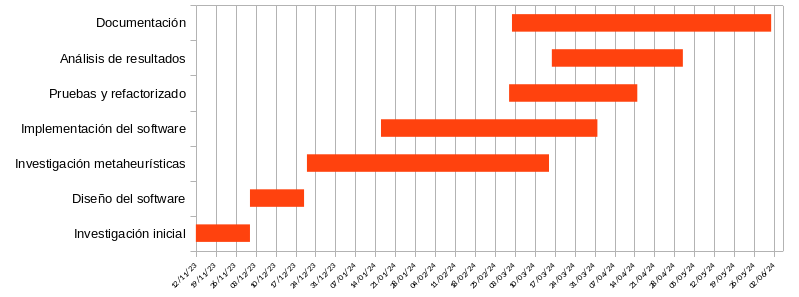
\includegraphics[width=1.2\textwidth]{imagenes/gantt-init.png}
      \end{center}
      \caption{Diagrama de Gantt inicial}
\end{figure}

La planificación inicial tiene en cuenta un curso ideal del ciclo de vida del proyecto, siendo las estapas más extensas la de creación del software e implementación de la documentación. Son etapas excluyentes, no pueden ocurrir a la vez según este tipo de planificación. Al terminar una etapa se pasa inmediatamente a la siguiente.\\[6pt]
La planificación final del proyecto se ha modificado significativamente debido a una serie de contratiempos y obstáculos surgidos durante su desarrollo, así como la influencia de numerosos eventos externos que han afectado a su cronograma. En particular, se han experimentado retrasos y bloqueos que han incidido en la duración prevista del proyecto. Por ejemplo, las etapas de implementación del software y la investigación de las metaheurísticas se han entrelazado debido a que la implementación efectiva del algoritmo se facilitaba una vez que se había estudiado a fondo la metaheurística correspondiente. Esto ha llevado a una reevaluación de la estrategia de planificación original, reconociendo que no habría sido eficiente estudiar todas las metaheurísticas simultáneamente y luego proceder con su implementación.

\begin{figure}[H]
      \begin{center}
      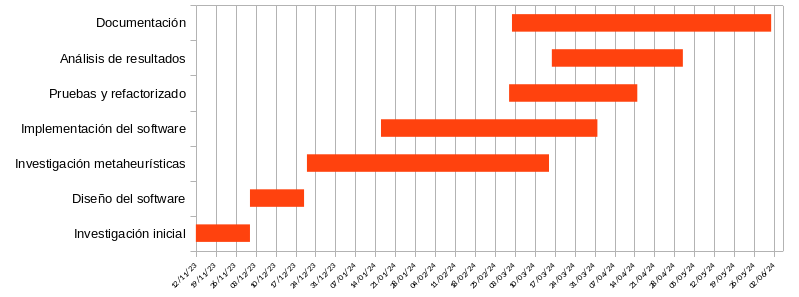
\includegraphics[width=1.2\textwidth]{imagenes/gantt-init.png}
      \end{center}
      \caption{Diagrama de Gantt final}
\end{figure}

El coste estimado del proyecto se divide en varios subcostes:
\begin{itemize}
      \item \textbf{Sueldo}: Teniendo en cuenta que el sueldo medio en España para un científico de datos es de $39.000$€~\cite{payscale_barcelona} al año y que el proyecto consta de un solo trabajador, se puede estimar un salario de $18.75$€/hora. 
\end{itemize}
%
%\chapter{Fundamentos Teóricos}
En este capítulo se describirán aquellos conceptos teóricos fundamentales para comprender el trabajo realizado en este proyecto.

\section{Optimización}
La optimización es un campo de estudio que trata, mediante el uso de las adecuadas herramientas matemáticas, de maximizar o minimizar una función objetivo. Esto significa, obtener la mejor solución posible para un problema dado dentro de un conjunto de alternativas y normalmente sujeto a una serie de restricciones que hacen de una solución satisfacible. Es un área interdisciplinar que aborda desde campos tales como la Economía, Ingeniería, Biología y muchas otras tantas disciplinas.\\[6pt]
La optimización es una disciplina arraigada en la naturaleza humana. Este impulso innato hacia la optimización ha llevado al desarrollo de diversas metodologías y técnicas a lo largo de la historia, desde los rudimentarios métodos de prueba y error hasta los sofisticados algoritmos de optimización computacional utilizados en la actualidad.

\subsection{Definición general de un problema de optimización}
Para poder convertir un problema abstracto en un problema de optimización concreto, con el que se pueda trabajar, es necesario establecer ciertos elementos fundamentales que lo definan de manera precisa y clara. En general, un problema de optimización se expresa de la siguiente forma~\cite{inbook}:

\begin{subequations}
    \begin{alignat}{2}
         & \text{Función objetivo a minimizar}                       & \qquad & f(x)\label{eq:optProb}                             \\
         & \text{Sujeto a} \nonumber                                                                                               \\
         & s \text{ restricciones de desigualdad}                    & \qquad & g_i(x)\leq 0, \quad j=1,2,...,s\label{eq:optProb2} \\
         & w \text{ restricciones de igualdad}                       & \qquad & h_j(x) = 0, \quad j=1,2,...,w\label{eq:optProb3}   \\
         & \text{Donde el número de variables es dado por} \nonumber & \qquad & x_i, \quad i=1,2,...,n
    \end{alignat}
\end{subequations}

La definición general de un problema de optimización proporciona una estructura sólida para abordar el problema abstracto. Establece la función objetivo que se busca minimizar o maximizar, junto con las restricciones que deben cumplirse. Estas restricciones pueden ser tanto desigualdades como igualdades, y todas juntas definen el \textbf{espacio de búsqueda} del problema.

\subsection{Función objetivo y función fitness}
Ambos términos, aunque a menudo se utilizan como sinónimos, desempeñan roles distintos en el ámbito de la optimización. La función \textit{objetivo}, como su nombre indica, establece el objetivo a alcanzar en la resolución del problema. Esta función cuantifica el rendimiento de las soluciones encontradas en relación con el objetivo específico del problema, que puede ser maximizar ganancias, minimizar distancia, entre otros objetivos. Por otro lado, la función de \textit{fitness}  evalúa la idoneidad de una solución dentro de una población de soluciones. Es decir, determina la calidad relativa de la solución respecto a otras alternativas.

Debe destacarse que la métrica de la función de \textit{fitness} suele ser estrictamente positiva, ya que representa la calidad de una solución, generalmente en un rango de valores entre $0$ y $1$. Por otro lado, la función objetivo puede ser positiva o negativa, dependiendo de si se busca maximizar o minimizar el objetivo. Además, la función de aptitud también puede llegar a ser una aproximación de la función objetivo, pero no necesariamente coinciden exactamente.\\[6pt]
Resumiendo, podría decirse que la función \textit{fitness} es un tipo particular de función objetivo que se utiliza como métrica de rendimiento~\cite{eiben2015}.

\subsection{Puntos globales o locales}
Se conocen como punto de óptimo global (mínimo o máximo) la solución (o vector hablando en términos matemáticos) cuyo valor para la función objetivo es el más grande en todo el espacio de soluciones posible, es decir, el espacio de búsqueda. Los puntos locales en cambio son varios, no solo uno como es el global. Son soluciones máximas o mínimas dentro de una región de soluciones.

\begin{figure}[H]
    \begin{center}
        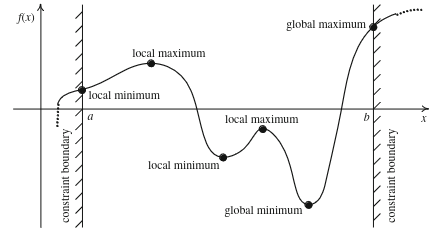
\includegraphics[width=1\textwidth]{imagenes/min-max_points.png}
    \end{center}
    \caption[Puntos globales y locales]{En esta figura extraída de \cite{inbook} puede observarse de manera intuitiva la diferencia entre punto global y puntos locales. El máximo global es el valor más alto para $f(x)$ en el espacio, mientras que un máximo global solo representa el valor más alto dentro de un ``vecindario"}
\end{figure}

Sea $f(x)$ una función a maximizar y $x^*$ una solución óptima. Un objetivo $G(x)$ está en su máximo global sí y solo si~\cite{inbook}:
\begin{equation}
    f(x^*) \geq f(x) \quad \forall x
\end{equation}
En cambio el objetivo está en un máximo local en el punto $x^*$ si:
\begin{equation}
    \begin{split}
        f(x^*) \geq f(x) \quad & \forall x \\
        & \text{dentro de un vecindario de } x^*\text{~\cite{inbook}}
    \end{split}
\end{equation}

\section{Teoría de la computación}
La teoría de la computación es un campo que estudia los fundamentos matemáticos y los límites de la computación. En esencia, se ocupa de preguntas fundamentales sobre qué se puede y qué no se puede computar, cómo se pueden resolver problemas de manera eficiente y qué tan difíciles son ciertos problemas en términos de recursos computacionales.\\[6pt]
Suele usarse la máquina de Turing, como modelo abstracto de computadora, para las demostraciones realizadas, creando un marco sencillo en el que entender cómo se ejecutan los algoritmos y cómo se resuelven estos.
\subsection{Máquina de Turing}
Una máquina de Turing, cuyo nombre proviene de su creador Alan Turing, es un modelo de computación matemático que es capaz de ejecutar algoritmos mediante el control de una serie de símbolos en la tira de una cinta y de acuerdo a una serie de reglas establecidas~\cite{stone1972}.\\[6pt]
Es capaz de general un modelo abstracto mediante el cual representar todo de algoritmos que resuelvan problemas computables.

\subsection{Grupos de complejidad P y NP}\label{complexity}
Se puede definir un lenguaje como una serie de cadenas dentro de un alfabeto, siendo este último un conjunto finito de símbolos~\cite{johnjeffery_automata}. \\[6pt]
Dada esta definición se dice que un lenguaje que es \textit{reconocible}, es decir, que una máquina de Turing puede determinar si una cadena pertenece al lenguaje o no, en un tiempo ``polinómico determinista" son conocidos como problema de la clase $P$. Que un problema sea resoluble en tiempo polinómico determinista en una máquina de Turing, significa que para cada estado solo existe una posible acción y que su tiempo de resolución puede expresarse como una función polinómica~\cite{johnjeffery_automata}. \\[6pt]
En contraposición, un problema de la clase $NP$ no es resoluble en tiempo polinómico determinista, sino en tiempo polinómico no determinista. Esto es, que puede resolverse expresando el tiempo como una función polinómica, pero con la diferencia de que el no determinismo implica que para pasar de un estado a otro es posible considerar múltiples acciones.\\[6pt]
La diferencia entre los problemas de las clases $P$ y $NP$ es fundamental en la teoría de la complejidad computacional. Mientras que los problemas de la clase $P$ son eficientemente resueltos, los problemas de la clase $NP$ pueden ser verificados en tiempo polinómico, pero su resolución en tiempo polinómico no está demostrada y tiende a ser exponencial.

\subsection{NP-Hard}
Un problema de decisión $H$ se considera $NP$-Hard o duro si, para cada problema $L$ en $NP$, hay una reducción de muchos a uno de tiempo polinómico de $L$ a $H$~\cite{leeuwen_algorithms_1998,johnjeffery_automata}. Esto significa que cualquier problema en $NP$ puede ser transformado en $H$ en tiempo polinómico, lo que sugiere que $H$ es al menos tan difícil como cualquier problema en $NP$.

\begin{figure}[H]
    \begin{center}
        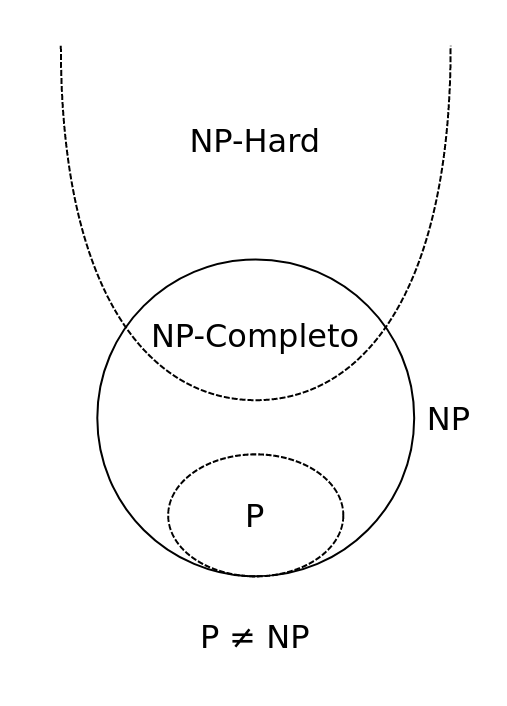
\includegraphics[width=0.6\textwidth]{imagenes/np_subsets.png}
    \end{center}
    \caption[Relación entre clases de complejidad]{En esta figura se puede ver la relación de pertenencia entre clases de complejidad. Puede observarse que $NP$-Hard no es un subconjunto de $NP$. Una solución para un problema $NP$-Hard podría transformarse mediante reducción y solucionar un problema $NP$, pero no siempre es así al revés.}
\end{figure}

\section{Selección de características}
La selección de características es un ejemplo de problema $NP$-Hard y uno de los problemas más importantes en el mundo de la inteligencia artificial, más concretamente en el \textbf{machine learning} o aprendizaje automático.

\subsection{Necesidad y motivo}
El aprendizaje automático se basa en los datos como fuente de aprendizaje. Es indispensable tener un buen conjunto de datos para poder obtener un modelo robusto y preciso. Por norma general o como se diría en inglés \textit{``as a rule of thumb''}, a más grande el conjunto de datos, mayor calidad del modelo. De hecho hay una correlación inmediata con esta sentencia.

\begin{figure}[H]
    \begin{center}
        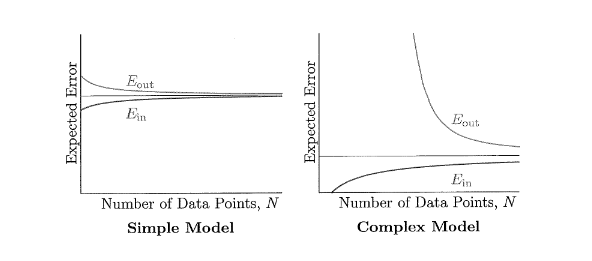
\includegraphics[width=1\textwidth]{imagenes/learning_from_data_vc.png}
    \end{center}
    \caption[Correlación entre error del modelo y N]{Esta figura extraída de \cite{Mostafa2012} visualiza la relación directa entre calidad del modelo (menos error esperado) y número de datos que se le proporciona al algoritmo de aprendizaje.}
    \label{fig:learning_from_data_vc}
\end{figure}

Es inmediato pensar que a mayor cantidad de datos, mejor calidad del modelo, y así es. Sin embargo, también existe una ``normal general'' que relaciona la complejidad del modelo y su capacidad de generalización. Es cierto que un modelo muy complejo (muchos parámetros) es capaz de ajustar mejor funciones más complejas, pero dentro de un conjunto con una serie de modelos suficientemente complejos, suele ser mejor idea elegir el más simple. Hay una serie clara de ventajas para ello:
\begin{enumerate}
    \item Menor  sensibilidad al sobre-ajuste.
    \item Mayor interpretabilidad del modelo y sus resultados.
    \item Mayor eficiencia y por tanto menor tiempo de ejecución y menor peso en memoria.
\end{enumerate}

De hecho, como puede observarse en la figura \ref{fig:learning_from_data_vc}, el modelo más complejo tiene un error esperado mucho mayor que el simple. El $E_{out}$ o error fuera de la muestra (error de generalización) es mucho más abrupto, es decir, generaliza peor.\\[6pt]
Por supuesto, con suficientes datos, con un $N$ (número de puntos) suficientemente grande, la tendencia del error es a la baja~\cite{Mostafa2012, shalev2014understanding}. Ocurre, sin embargo, que la recolección, limpieza y transformación de datos es una tarea compleja, por ello es mejor ceñirse, de nuevo, a el modelo más pequeño que obtenga una solución con suficiente calidad.

\subsection{Concepto}
El funcionamiento y motivo es explicado ya en la definición del problema en \ref{def_problem}. Por evitar redundancias se procede a explicar el concepto de manera abreviada y puntualizando en los apartados más importantes.\\[6pt]
La selección de características es una conocida y necesaria técnica de pre-procesamiento de datos para la construcción de un modelo de aprendizaje. Su función es escoger un subconjunto óptimo de características dentro del conjunto inicial, de forma que la complejidad del modelo se reduzca.\\[6pt]
Este problema es del tipo $NP$-Hard, como ya se ha mencionado previamente en \ref{def_problem} y explicado en \ref{complexity}.
La selección de características ayuda a una serie de factores como son la interpretabilidad, mejora de la eficiencia temporal y espacial del modelo y sobre todo con la \textbf{maldición de la dimensionalidad}~\cite{venkat2018curse, bellman1957dynamic}.

\subsection{Maldición de la dimensionalidad}
El término fue acuñado por Bellman en $1961$~\cite{bellman1961adaptive}. Este fenómeno ocurre cuando la dimensionalidad de los datos es muy grande. En un espacio de características de alta dimensión, es común que los datos estén muy dispersos, lo que significa que hay muy pocos datos en comparación con la cantidad posible de características. Esto dificulta que los modelos representen correctamente todo el espacio de características~\cite{peng_interpreting_2024}.

\begin{figure}[H]
    \begin{center}
        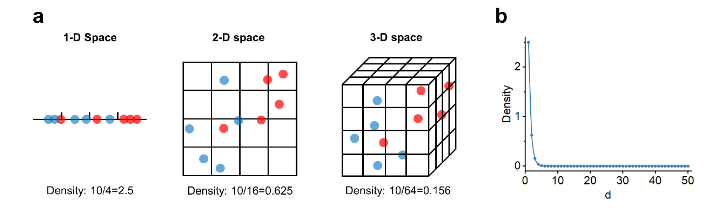
\includegraphics[width=1\textwidth]{imagenes/curse-dimen-example.png}
    \end{center}
    \caption[Tendencia de incremento de dimensionalidad en varios espacios de características]{Esta figura extraída de \cite{peng_interpreting_2024} muestra la tendencia en la densidad a medida que se incrementa la dimensionalidad del espacio. En $(a)$ se muestra la densidad con diez puntos de datos en un espacio $1D$, en $(b)$ se muestra la tendencia al incrementar las dimensiones.}
\end{figure}

Además, en espacios de alta dimensión, la medición de distancias puede volverse inválida. Esto se debe a que las distancias entre puntos de datos diferentes tienden a converger a un mismo valor a medida que aumenta la dimensionalidad. Esto significa que las medidas de distancia ya no son tan útiles para medir la similitud entre datos~\cite{peng_interpreting_2024, venkat2018curse}. En el trabajo de Beyer y compañeros~\cite{beyer99nn} se observó como esto ocurría y por tanto un escaneo lineal (recorrer los puntos uno a uno) resultaba en altas dimensiones más práctico que otras técnicas complejas.
\section{Metaheurísticas}
Dentro de la optimización hay muchos tipos de métodos, dentro de los pseudoaleatorios pueden encontrarse las metaheurísticas. Estas son algoritmos basados en una abstracción de mayor nivel de la \textbf{heurísticas}. Mientras que las heurísticas se apoyan en el conocimiento específico del campo en el que se encuentra el problema, y están restringidas a su dominio, las metaheurísticas son aplicables a todo tipo de problemas, independientemente de su área de optimización~\cite{bianchi2009survey}. Es cierto que hay algoritmos que son más convenientes para ciertos problemas que otros, pero su aplicación es generalizada. Normalmente, las metaheurísticas son diseñadas a siguiendo una inspiración en la naturaleza, ya sea en fenómenos físicos o en el comportamiento animal. Ejemplo de estos son algoritmos como el \textit{Búsqueda Cuckoo}, \textit{Enfriamiento Simulado} o incluso \textit{Algoritmos Genéticos}.\\[6pt]
Las metaheurísticas son especialmente útiles en problemas cuya resolución no es factible debido a altos costos computacionales, ya sea porque es posible analíticamente pero computacionalmente costoso, o porque el problema no es abordable mediante algoritmos convencionales. Son capaces de encontrar óptimos locales lo suficientemente aceptables, soluciones no óptimas, pero si muy buenas~\cite{bianchi2009survey}.

\begin{figure}[H]
    \begin{center}
        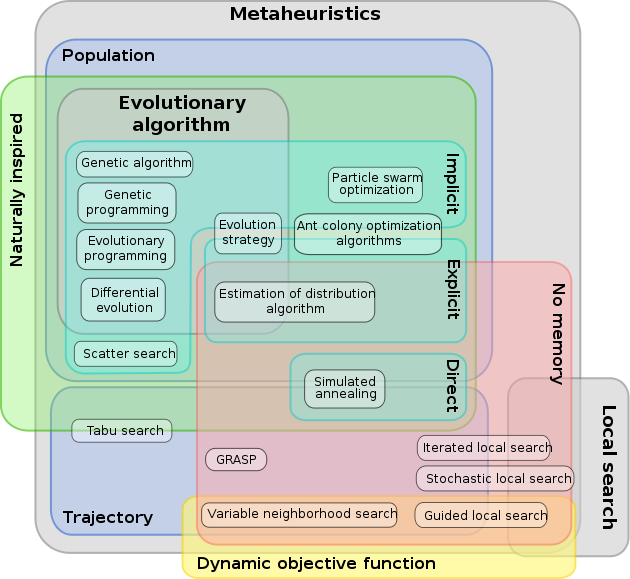
\includegraphics[width=0.8\textwidth]{imagenes/mh_euler_graph.png}
    \end{center}
    \caption[Clasificación metaheurísticas]{En esta figura de los autores Johann ``nojhan'' Dréo y Caner Candan, se clasifican las distintas metaheurísticas por inspiración.}
\end{figure}

\subsection{Exploración vs explotación}
Las metaheurísticas, y algoritmos basados en técnicas pseudoaleatorias, deben tener un balance entre sus factores explorativos y explotativos. De no ser así, los algoritmos tendrían tendencias a la convergencia temprana, dejando de lado mucho espacio por explorar y por ende soluciones posiblemente mejores (estancamiento en óptimos locales) o serían muy lentos en la convergencia hacia una solución.\\[6pt]
La \textbf{exploración} se refiere a la habilidad del algoritmo de buscar nuevas y diversas regiones en el espacio de búsqueda/solución. Es una característica de la búsqueda global, que también puede ser llamada \textit{diversificación}. En cambio, la explotación es la habilidad de la búsqueda de explotar las mejores soluciones encontradas hasta el momento y mejorarlas localmente, dentro de un ``vecindario''~\cite{xu2014exploration}.\\[6pt]
No existe un equilibrio \textit{de facto} entre exploración y explotación en las metaheurísticas. Aún no se ha alcanzado una respuesta definitiva a esta cuestión. Desde una perspectiva de sistemas, una metaheurística puede entenderse como un sistema dinámico compuesto por numerosos ``individuos'' que interactúan entre sí. Estos individuos representan las distintas soluciones o posiciones en el espacio de búsqueda que la metaheurística explora~\cite{6896450}. Las interacciones entre estos individuos son las que conforman comportamientos explorativos o explotativos y dependen del problema a solucionar y del propio algoritmo su equilibrio.

\section{Teorema No Free Lunch}
El Teorema de ``No Free Lunch'' (NFL) establece que, en promedio, ningún algoritmo de búsqueda puede superar a otros algoritmos en la búsqueda de todas las funciones objetivo posibles. En otras palabras, no existe un algoritmo universalmente óptimo que pueda dominar en todos los problemas de búsqueda. Esto implica que, si un algoritmo es efectivo para un conjunto particular de problemas, es probable que no lo sea para otros~\cite{585893}.\\[6pt]
Relacionar este teorema con las metaheurísticas implica reconocer que no hay una única metaheurística que sea la mejor para todos los problemas de optimización. Cada problema puede tener características únicas que lo hacen más o menos adecuado para ciertas metaheurísticas. Por lo tanto, en lugar de buscar una solución universal, las metaheurísticas se centran en explorar y explotar diferentes áreas del espacio de búsqueda para encontrar soluciones aceptables o incluso óptimas para problemas específicos.\\[6pt]
Pese a ello, las suposiciones de este tipo de teoremas, como conjuntos de datos extraídos de una distribución uniforme sobre todos los conjuntos de datos posibles, están completamente desalineadas con el mundo real, donde los datos suelen ser altamente estructurados y no están uniformemente muestreados~\cite{goldblum2023free}.\\[6pt]
De esta forma y faltando evidencia concluyente al respecto, es interesante mencionar el \textbf{NFL}, pero sin llegar a negar la posibilidad de nuevas y más precisas interpretaciones.

\section{Aprendizaje automático}
El aprendizaje automático es una sub-rama de estudio de la inteligencia artificial o \textbf{IA}, la cual aglomera una serie de métodos que pueden, de manera automática, detectar patrones en conjuntos masivos de datos para predecir datos futuros~\cite{murphy2012machine}. El aprendizaje automático o \textit{machine learning} en inglés, es usado en una amplia variedad de campos por su utilidad trasversal. Algunos de ellos son la agricultura, marketing, videojuegos, meteorología, física, etc.\\[6pt]
Los algoritmos de aprendizaje automático son capaces de encontrar patrones en los datos, como ya se ha mencionado. Por ello, es necesario nutrir a estos algoritmos con datos de calidad. Un modelo de aprendizaje automático será tan bueno como los datos que se le puedan proveer, no más. De esta forma la recoleción de datos y su procesamiento se convierten en una prioridad a la hora de crear modelos.\\[6pt]
Hay muchas formas de estructurar los datos y muchos tipos de algoritmos acorde a estos ``inputs''. En este documento se tratará con información en formato tabular, es decir, información en tablas con filas y columnas, donde cada fila representa un registro de información y cada columna una característica asociada. Esta última es la que determinará la complejidad del modelo. 

\subsection{Aprendizaje supervisado}
Este subtipo de aprendizaje automático se caracteriza por tener un conjunto de datos sobre los que se entrena y una salida esperada (etiquetas) para cada punto de los datos~\cite{sah2020machine}. Es bastante costoso porque etiquetar cada dato es una tarea laboriosa y poco escalable.

\begin{figure}[H]
    \begin{center}
        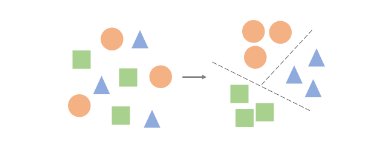
\includegraphics[width=1\textwidth]{imagenes/ml-supervised-learning.png}
    \end{center}
    \caption[Aprendizaje supervisado]{Figura extraída de \cite{sah2020machine} que muestra un ejemplo de aprendizaje supervisado.}
\end{figure}

\subsection{Aprendizaje no supervisado}
Cuando los datos solo vienen en forma de entrada y no se tiene ninguna salida (no hay etiquetas) entonces se trata de un aprendizaje no supervisado. Los algoritmos de este tipo se basan en la diferenciación de los datos mediante los patrones subyacentes que puedan encontrar. Son comunes en el aprendizaje no supervisado los algoritmos de \textit{clustering}~\cite{sah2020machine}.

\begin{figure}[H]
    \begin{center}
        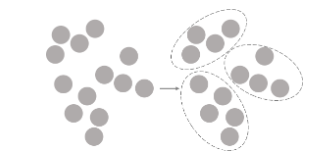
\includegraphics[width=0.7\textwidth]{imagenes/ml_unsupervised-learning.png}
    \end{center}
    \caption[Aprendizaje no supervisado]{Figura extraída de \cite{sah2020machine} que muestra un ejemplo de aprendizaje no supervisado. Se trata de dividir en clústers sin información de etiquetas.}
\end{figure}

\subsection{SVM}
Las máquinas de vectores de soportes o \textit{SVM} fueron introducidas por primera vez en~\cite{cortes_support-vector_1995}. En este documento será uno de los algoritmos de clasificación usados en la función \textit{fitness} para cuantificar la calidad de los pesos aprendidos por los algoritmos optimizadores.\\[6pt]
Las máquinas de vectores de soporte son algoritmos cuya principal característica se basa en la creación de un hiperplano o conjunto de hiperplanos en un espacio $n$-dimensional~\cite{scikit-learn-svm,}. Este hiperplano o hiperplanos es elegido de manera que maximice el margen entre los puntos de datos de todas las clases a predecir. El margen es la distancia entre el hiperplano y los puntos de datos más cercanos de cada clase, estos puntos se denominan vectores de soporte. De esta manera se consigue minimizar el error de generalización~\cite{hastie2009elements}.\\[6pt]
La idea más intuitiva es, que al haber más espacio entre los puntos de distintas clases, hay más posibilidad de que los puntos no vistos, los puntos a predecir, caigan en zonas correctas.

\begin{figure}[H]
    \begin{center}
        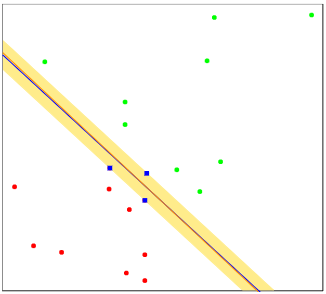
\includegraphics[width=0.5\textwidth]{imagenes/svm-margin.png}
    \end{center}
    \caption[Margen en SVM]{Figura extraída de \cite{hastie2009elements} en la que se muestra de forma gráfica en un espacio $2$-dimensional el margen óptimo de separación de dos clases.}
\end{figure}

\subsection{K-nearest neighbors}
El algoritmo de $k$ vecinos más cercanos fue presentado en \cite{fix_discriminatory_1989} por Evelyn Fix y Joseph Hodges, y más tarde ampliado en \cite{cover_nearest_1967} por Thomas Cover.\\[6pt]
Puede ser utilizado para regresión o clasificación, pero su uso suele darse más en este último problema. Este algoritmo ofrece una premisa sencilla, la clase de un punto $p$ dependerá de cuál sea la clase mayoritaria dentro del subconjunto de $k$ vecinos más cercanos~\cite{10.1007/978-3-540-39964-3_62}.\\[6pt]
Valores mayores de $k$ incrementan la varianza, pero decrementan el sesgo (equilibrio sesgo-varianza~\cite{Mostafa2012}). De forma inversa, a menor $k$ mayor sesgo y menor varianza.\\[6pt]
Otra forma de verlo es que si $k=1$ (el valor mínimo), el modelo entrenado será muy complejo, pues cada punto puede variar de clase por mínimo que sea el cambia en su entorno. Es un modelo que tiende a sobre-ajustar. Con $k=n$ el modelo es lo más simple posible, al tener en cuenta absolutamente todos los puntos, la clasificación será siempre la de la clase más repetida.
% %
%\chapter{Estado del arte}
La selección de características es un problema cuya popularidad ha ido en aumento con el paso de los años. No es algo casual, pues la cantidad de datos recogidos para tareas de aprendizaje automático y áreas derivadas, como el aprendizaje profundo, ha ido en aumento de manera casi exponencial.

\begin{figure}[H]
    \begin{center}
        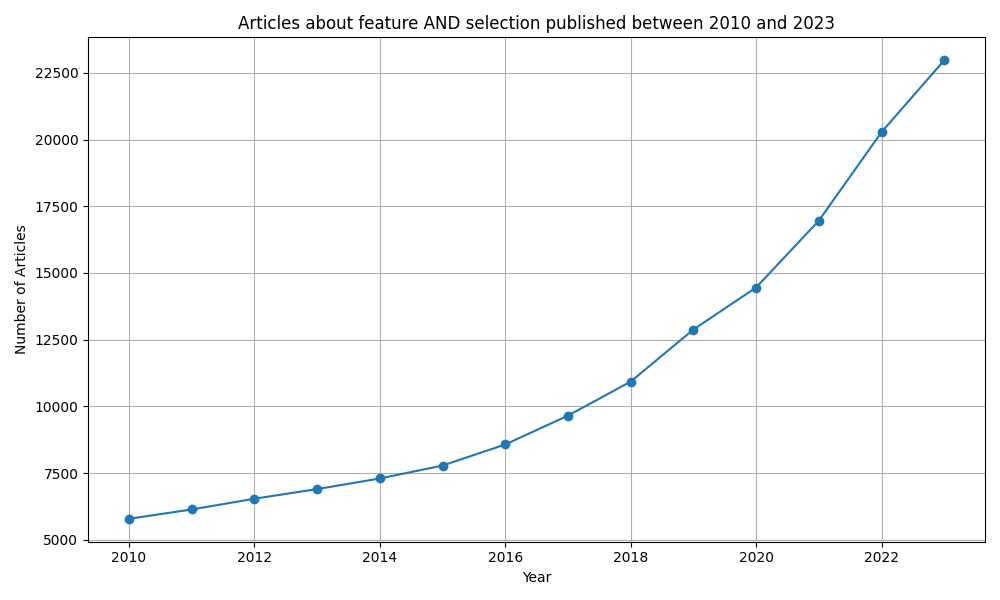
\includegraphics[width=1\textwidth]{imagenes/scopus_chart.png}
    \end{center}
    \caption[Popularidad de feature selection sobre los años]{En esta figura se muestra el número de artículos publicados relacionados con la selección de características. Se ha usado el buscador Scopus para estos resultados.}
    \label{fig:pop_fs}
\end{figure}

También se puede observar una tendencia  prácticamente igual en la popularidad sobre los años del problema de selección de características, pero abordado con técnicas metaheurísticas.

\begin{figure}[H]
    \begin{center}
        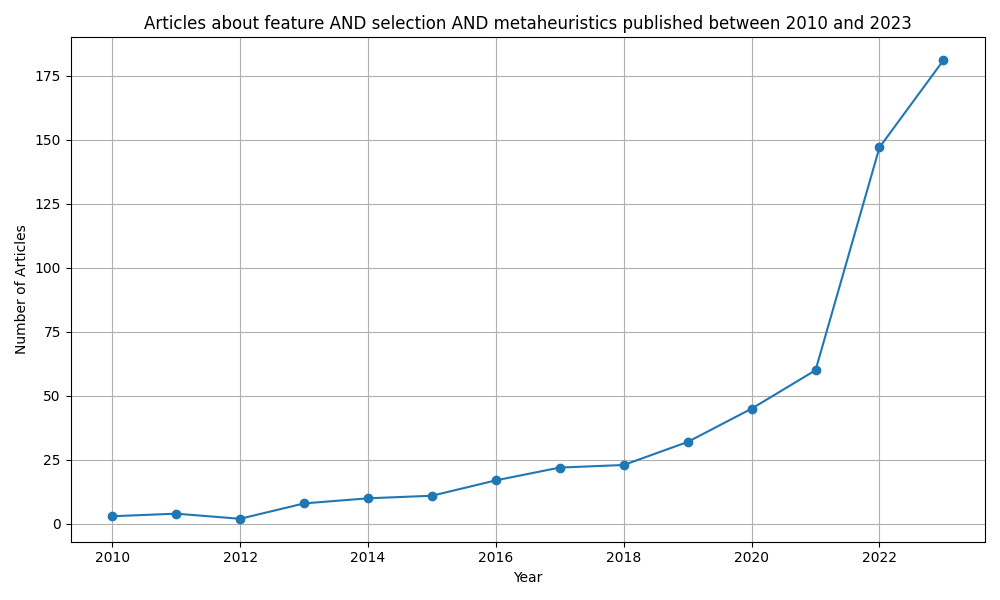
\includegraphics[width=1\textwidth]{imagenes/scopus_chart2.png}
    \end{center}
    \caption[Popularidad de feature selection + metaheuristics sobre los años]{De igual forma que en la figura \ref{fig:pop_fs} las mateheuristicas han ido muy ligadas a la resolución de este problema. Se ha usado el buscador Scopus para estos resultados.}
\end{figure}

Y es que las metaheurísticas son algoritmos muy convenientes en la resolución de este tipo de problemas. Algoritmos analíticos no son válidos cuando el conjunto de datos tiene un número de características muy elevado debido a una cantidad de combinaciones simplemente inabordable en términos computacionales. Debido a ello, se suelen utilizar algoritmos más rápidos cuya solución no es óptima en términos globales, pero si suficientemente buena.\\[6pt]
Muchos algoritmos metaheurísticos han sido propuestos a lo largo de los años. Se han escogido los más destacables en cuanto a resultados y más mencionados entre todos ellos, dando una selección de algoritmos metaheurísticos modernos de, en principio, muy alta calidad. No solo son seleccionados algoritmos modernos, sino que también se han escogido una serie de algoritmos más ``clásicos'', pero cuya aplicación es más extendida y con resultados que, de forma empírica, han demostrado ser más que buenos a lo largo de décadas de uso.

\begin{table}[H]
    \parbox{.45\linewidth}{
        \centering
        \begin{tabular}{l}
            \hline
            Algoritmos \\ \hline
            GWO        \\
            FA         \\
            GOA        \\
            WOA        \\
            DA         \\
            CS         \\
            BA         \\
            \hline
        \end{tabular}
        \caption{Algoritmos modernos}
    }
    \hfill
    \parbox{.45\linewidth}{
        \centering
        \begin{tabular}{l}
            \hline
            Algoritmos \\ \hline
            PSO        \\
            GA         \\
            ACO        \\
            DE         \\
            ABCO       \\
            \hline
        \end{tabular}
        \caption{Algoritmos clásicos}
    }
\end{table}
Para aclarar ciertas cuestiones referentes a las soluciones en este tipo de algoritmos estocásticos de tipo evolutivo, si no se especifica un tipo de representación se da por hecho que las soluciones se representan como vectores en un espacio $n$-dimensional. Un conjunto de individuos/vectores dan como resultado una población. La población es una matriz de $N\times M$, donde $N$ es el número de filas o número de individuos en la población y $M$ es el número de características del problema ($M$ dimensiones). Algunos algoritmos admiten codificación binario y otros continua, ese tipo de cuestiones si serán especificadas.
\section{Algoritmos genéticos}
\subsection{Introducción}
Los algoritmos genéticos están inspirados en la selección natural y se utilizan tanto en problemas de optimización con restricciones como sin ellas. Es una metaheurística que modifica una población de soluciones individuales de manera repetida, seleccionando soluciones ``padre'' que dan lugar a la siguiente generación de soluciones en la siguiente iteración del algoritmo. En su forma más básica, un algoritmo genético opera sobre una población de soluciones potenciales a un problema dado. Cada solución potencial, a menudo llamada individuo o cromosoma, está representada como una cadena de símbolos, que puede ser binaria, numérica o simbólica~\cite{10.5555/522098}.

\subsection{Funcionamiento y Operadores}
Las soluciones o \textbf{fenotipos} están compuestas por una serie de propiedades, características, cromosomas o \textbf{genotipos}, que pueden ser mutados y alterados. La representación más común es la binaria, pero otras codificaciones son posibles.

El proceso típico incluye~\cite{mathew2012genetic}:
\begin{itemize}
    \item Inicialización aleatoria de la población.
    \item Evaluación del \textit{fitness} de cada individuo.
    \item Selección de padres basada en el \textit{fitness}.
    \item Creación de una nueva generación mediante cruces y mutaciones.
    \item Elitismo: selección de los mejores individuos~\cite{mirjalili2019genetic}.
\end{itemize}

\begin{figure}[H]
    \begin{center}
        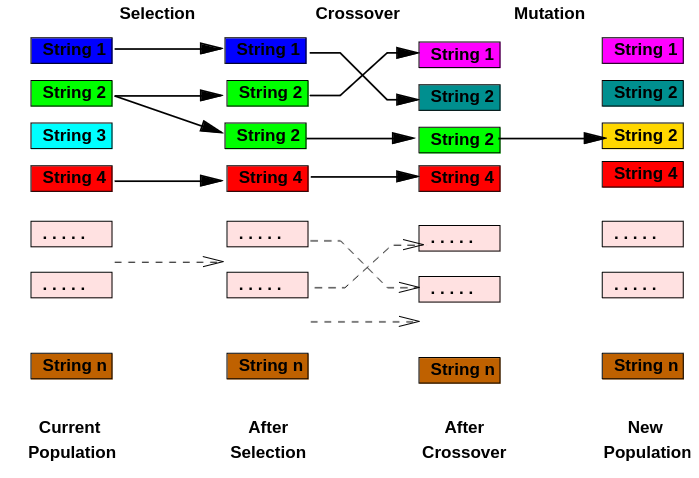
\includegraphics[width=0.6\textwidth]{imagenes/ga-working-principle.png}
    \end{center}
    \caption[Funcionamiento de un algoritmo genético]{Figura obtenida de \cite{mathew2012genetic}}
\end{figure}


El algoritmo termina cuando se alcanza cierta tolerancia de error o número máximo de iteraciones.

\subsubsection{Selección}
La selección se puede llevar a cabo con varios métodos, uno de los más utilizados en selección por torneo.\\[6pt]
En la selección por torneo, los individuos compiten entre sí en grupos pequeños. Cada grupo (torneo) tiene varios competidores (individuos). El competidor con la mejor aptitud (\textbf{fitness}) dentro del grupo tiene más probabilidad de ganar. Los ganadores son seleccionados para ``reproducirse''. Este proceso se repite hasta que se completa el \textit{pool} de apareamiento con los ganadores de los torneos~\cite{miller_genetic_nodate}. La probabilidad de cada individuo en base a su \textbf{fitness} se calcula de la siguiente manera:
\begin{equation}
    P(\text{parent}_i) = \frac{\text{fitness}(\text{parent}i)}{\sum_{j=1}^{N} \text{fitness}(\text{parent}_j)}
\end{equation}

\subsubsection{Cruce}
Existen múltiples tipos de crossover o cruces. Se describen los dos usados en este proyecto (uno para la versión binaria del algoritmo y otra para la real):
\begin{itemize}
    \item \textbf{One-point crossover}: Se elige al azar un punto en los cromosomas de ambos progenitores y se designa como "punto de cruce". Los bits a la derecha de ese punto se intercambian entre los dos cromosomas parentales. El resultado son dos descendientes, cada uno con información genética de ambos progenitores~\cite{DAGDIA2020283}.
          \begin{figure}[H]
              \begin{center}
                  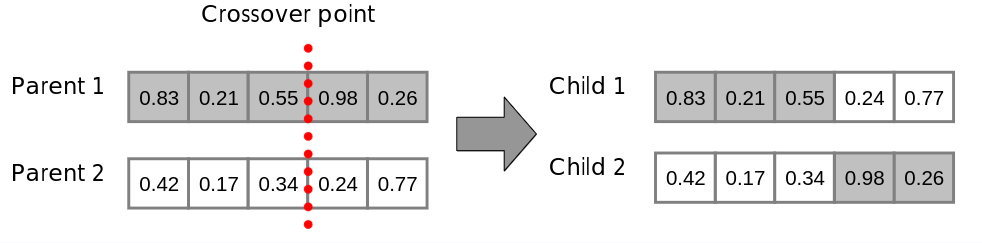
\includegraphics[width=0.6\textwidth]{imagenes/one-point-crossover.png}
              \end{center}
              \caption[One point crossover]{One-point crossover~\cite{purduelecture}}
          \end{figure}
    \item \textbf{Blend crossover}: Dado dos números reales para cada uno de los genes de los padres al hijo se le asignará un número aleatorio entre ese rango de gen para cada gen que conforme al vector cromosómico~\cite{purduelecture}.
          \begin{figure}[H]
              \begin{center}
                  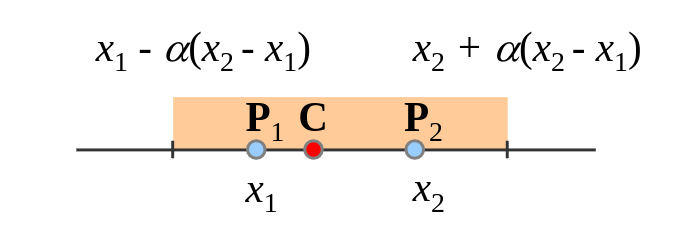
\includegraphics[width=0.6\textwidth]{imagenes/blend-crossover.png}
              \end{center}
              \caption[Blend crossover]{Blend crossover~\cite{purduelecture}}
          \end{figure}
\end{itemize}

\subsubsection{Mutación}
Su propósito es mantener la diversidad genética de los cromosomas de una población de un algoritmo evolutivo.
El operador más básico y clásico consiste en cambiar un bit arbitrario de un genotipo o solución de un algoritmo genético binario a su estado inverso dada una probabilidad de mutación~\cite{mirjalili2019genetic}.

\subsubsection{Elitismo}
El elitismo garantiza que las soluciones de alta calidad sobrevivan en las generaciones futuras, ayudando en la explotación del espacio de búsqueda. La cantidad de individuos élite seleccionados debe ser elegida con precisión~\cite{mirjalili2019genetic}.

\section{Algoritmos de colonias de hormigas}
\subsection{Introducción}
El algoritmo de colonia de hormigas o \textbf{ACO} es una técnica probabilística que trata de resolver problemas computacionales que pueden ser reducidos a la búsqueda de caminos óptimos a través de grafos. Se basa en el comportamiento de las hormigas reales y su comunicación vía feromonas. Las hormigas vagan por el mundo en búsqueda de comida de forma aleatoria. Cuando estas encuentran comida, dejan trazas de feromonas en su camino, de esta forma, si otras hormigas encuentran ese rastro, se hace más probable que recorran ese camino y dejen de vagar de forma aleatoria. Sin embargo, las trazas de feromonas se evaporan con el tiempo, perdiendo su fuerza de atracción sobre otras hormigas. De esta forma, si el camino es muy largo, la hormiga tardará mucho en recorrerlo y la traza de feromonas tendrá más tiempo a evaporarse. De manera análoga, a más corto es el camino, más rápido se recorre y más densidad de feromonas acumula~\cite{kashef_advanced_2015}.

\subsection{Funcionamiento y Operadores}
Para poder adaptar el algoritmo ACO a un problema es necesario reducir ese problema a la búsqueda del camino más corto dentro de un grafo ponderado. De esta forma, la \textbf{representación} en este tipo de algoritmo debe ser la de un grafo.
Cada característica del problema original se representa como un nodo $n$. Los caminos que conectan a los nodos ($e$) representan la elección del subconjunto de características. El camino deberá ser lo más corto posible maximizando a su vez el \textbf{accuracy}~\cite{kashef_advanced_2015}.

\subsubsection{Regla de transición probabilística}
\begin{equation}
    P_{ij}^k(t)=\begin{cases} \frac{\tau_{ij}^{\alpha}\eta_{ij}^{\beta}}{\sum_l\tau_{il}^{\alpha}\eta_{il}^{\beta}} & \text{Si $l$ y $k$ son nodos admisibles} \\ 0 & \text{De lo contrario} \end{cases}
\end{equation}
Donde:
\begin{itemize}
    \item $P_{ij}^k(t)$ denota la probabilidad de transición de un nodo de $i$ a $j$ en la $k$-hormiga (agente) en el instante de tiempo $t$.
    \item $\tau_{ij}$ es la cantidad de traza de feromona en la arista $(i,j)$ en el momento $t$. $\eta_{ij}$ es la heurística de deseabilidad o visibilidad de la arista.
    \item $\beta$ y $\alpha$ son dos parámetros que controlan la importancia relativa del valor de la feromona vs la información de la heurística.
\end{itemize}

\subsubsection{Evaporación de feromona}
Después de que todas las hormigas hayan terminado su camino, la evaporación de feromonas comienza. El contenido de feromonas del camino $(i,j)$ en el instante $t+1$ es:
\begin{equation}
    \tau_{ij}(\text{new})=(1-p)\tau_{ij}(t)+\sum_{k=1}^m\Delta\tau_{ij}^k(t)+\Delta\tau_{ij}^g(t)
\end{equation}
Donde:
\begin{itemize}
    \item $\Delta\tau_{ij}^k=\begin{cases}\frac{Q}{F^k}&\hspace{6mm}\text{Si la hormiga k pasa por la arista (i,j) en }T^k\\0 &\hspace{6mm}\text{De lo contrario}\end{cases}$
    \item $p\in (0,1]$ es el ritmo de evaporación.
    \item $m$ es el número de hormigas.
    \item $\Delta\tau_{ij}^k$ y $\Delta\tau_{ij}^g$ son respectivamente, la cantidad de feromonas colocadas en la arista $(i,j)$ por la hormiga $k$ y la cantidad de feromonas depositadas por la mejor hormiga $g$ en el instante $t$ sobre la arista $(i,j)$.
    \item $Q$ es una constante y $F^k$ es el valor de coste de la solución encontrada por la hormiga $k$ en el tour $T^k$, es decir, $F^k$ es el \textit{fitness} de la hormiga $k$.
\end{itemize}
Se utiliza el sistema \textit{max-min}, solo la mejor hormiga puede depositar feromona.\\[6pt]
En el algoritmo original, no había heurística de deseabilidad o visibilidad ($\eta$), solo información en términos de feromona~\cite{dorigo_ant_1999}.

\section{Optimización por enjambre de partículas}
\subsection{Introducción}
El algoritmo conocido como optimización por enjambre de partículas o en inglés \textit{particle swarm optimization} fue concebido en $1995$ por James Kennedy y Russel Eberhart~\cite{kennedy_particle_1995}. En este algoritmo, un conjunto de soluciones candidatas, llamadas partículas, se mueven en un espacio de búsqueda multidimensional. Cada partícula ajusta su posición de acuerdo con su experiencia personal y la experiencia del grupo.

\subsection{Funcionamiento y Operadores}
Las soluciones son descritas como individuos dentro de un enjambre (conjunto total de posibles soluciones) que tienen una posición y una velocidad en todo momento. La posición de estos individuos representa la solución en sí.

\subsubsection{Velocidad}
\begin{equation}
    v_{i}(t+1) = v_{i}(t) + c_1 \cdot \text{rand}() \cdot (pbest_{i} - x_{i}(t))+ c_2 \cdot \text{rand}() \cdot (gbest - x_{i}(t))
\end{equation}

Donde:
\begin{itemize}
    \item $v_{i}(t+1)$ es la velocidad de la partícula $i$ en la siguiente iteración.
    \item $v_{i}(t)$ es la velocidad de la partícula $i$ en la iteración actual.
    \item $c_1$ y $c_2$ son factores de aceleración que controlan la influencia de las mejores posiciones.
    \item $\text{rand}()$ es un número aleatorio en el rango [0, 1].
    \item $pbest_{i}$ es la mejor posición histórica de la partícula $i$.
    \item $x_{i}(t)$ es la posición actual de la partícula $i$ en la iteración $t$.
    \item $gbest$ es la mejor posición global del grupo.
\end{itemize}

\subsubsection{Posición}

\begin{equation}
    x_{i}(t+1) = x_{i}(t) + v_{i}(t+1)
\end{equation}

Estas ecuaciones se utilizan para guiar el movimiento de las partículas a través del espacio de búsqueda hacia las mejores soluciones, adaptándose tanto a la mejor solución encontrada por la propia partícula ($pbest$) como a la mejor solución encontrada por cualquier partícula en el enjambre ($gbest$)~\cite{kennedy_particle_1995}. Con el tiempo, las partículas tienden a converger hacia las mejores soluciones conocidas.

\section{Evolución diferencial}
La evolución diferencial surgió como un algoritmo de optimización para problemas no diferenciables y no lineales, con pocas variables de control, robusto, paralelizable y muy eficaz. El algoritmo de evolución diferencial o \textit{differential evolution} en inglés fue diseñado para resolver problemas continuos, a diferencia del propósito original de su ``hermano gemelo'' el algoritmo genético, cuya finalidad inicial era resolver problemas binarios. Este algoritmo fue presentado en $1996$ por Storn y Price en \cite{storn_differential_1997}.\\[6pt]
En la evolución diferencial, la diferencia de vectores es un concepto clave que se utiliza en el operador de mutación. Esta se calcula restando dos vectores de la población. Gracias a esta operación puede calcularse la distancia entre vectores y esto conlleva una serie de ventajas~\cite{storn_differential_1997}:
\begin{itemize}
    \item Las posiciones de los individuos proporcionan información ya que si los individuos están bien distribuidos (y si la población es lo suficientemente grande), la población inicial será una buena representación de todo el espacio de búsqueda.
    \item Las distancias entre estos individuos serán inversamente proporcionales al tamaño de la población.
    \item A medida que avanza la búsqueda y los individuos comienzan a converger hacia un óptimo local, las distancias entre los individuos comenzarán a disminuir.
\end{itemize}

\subsection{Funcionamiento y Operadores}
La representación suele ser la misma que en otros algoritmos metaheurísticos. DE fue diseñado para optimizar un problema continuo, por lo que la población debería ser un conjunto de números reales.

\subsubsection{Mutación}
La operación de mutación produce un vector, conocido como vector de prueba o en inglés \textit{trial vector}. Para ello se hace uso de un vector objetivo y una diferencia de vectores ponderada. La mutación elige a un padre $x_{i}$, generando un vector de prueba $u_{i}$ siguiendo lo siguientes pasos:
\begin{enumerate}
    \item Se selecciona un vector objetivo $x_{i_1}$ tal que $i\neq i_1$.
    \item Se selecciona aleatoriamente dos individuos $x_{i_2}$ y $x_{i_3}$ de la población tal que $i\neq i_1\neq i_2\neq i_3$ y $i_2,i_3$ sean seleccionados con una probabilidad uniforme. Es necesario que todos los individuos tengan la misma probabilidad de selección.
\end{enumerate}
Finalmente, se calcula el vector de prueba:
\begin{equation}
    u_i = x_{i_1}+\beta\dot(x_{i_2}-x_{i3})
\end{equation}
Donde $\beta$ es un factor de escalado que controla la amplificación de la variación diferencial (mutación más diversa/grande)~\cite{storn_differential_1997}.

\begin{figure}[H]
    \begin{center}
        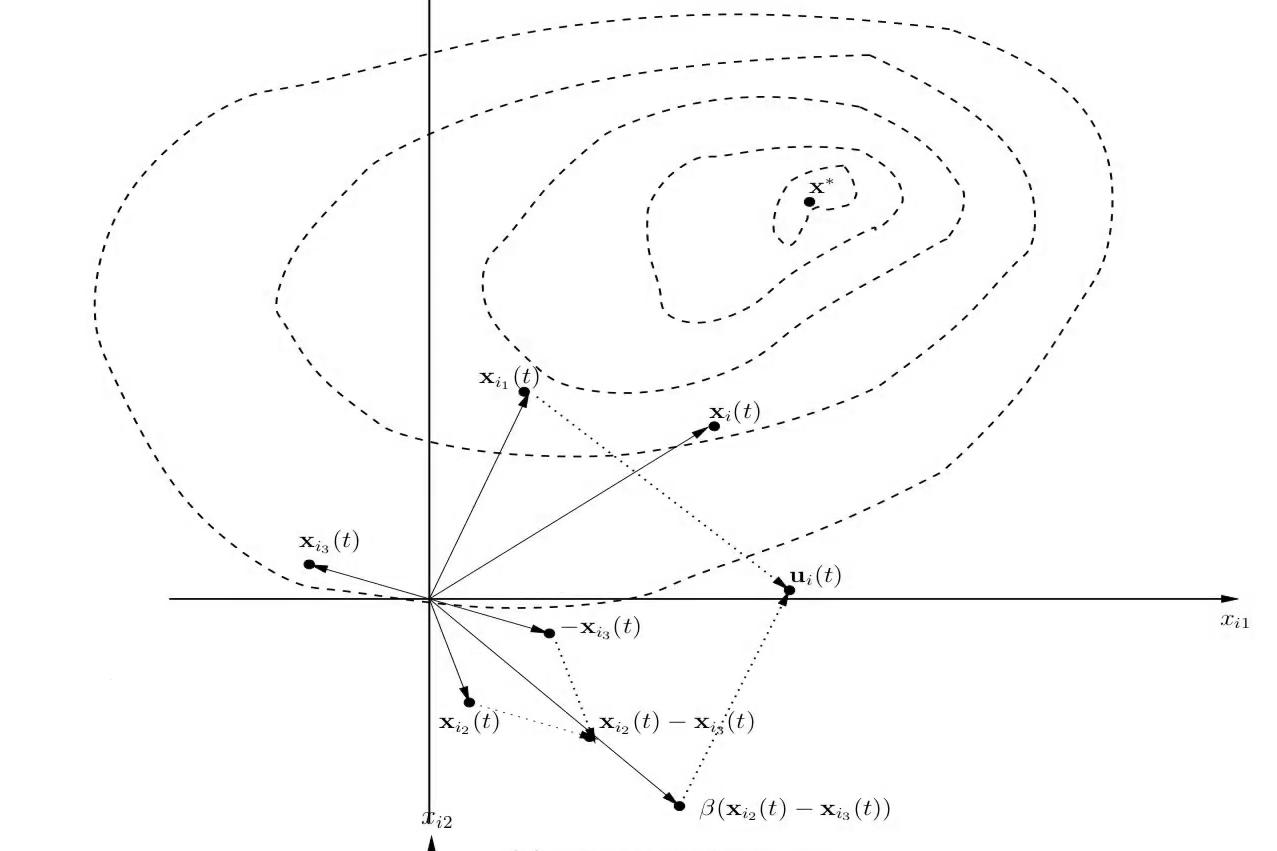
\includegraphics[width=1\textwidth]{imagenes/de-mutation.png}
    \end{center}
    \caption[Mutación en DE]{Esta figura ha sido seleccionada de \cite{10.5555/1557464}. Muestra de manera gráfica en un espacio bidimensional como funciona el operador de mutación y cómo se crea el ``trial vector''.}
\end{figure}

Una ventaja que tiene el uso de diferencias de vectores en la mutación, es que si todos lo individuos tienen la misma probabilidad de selección, la media de la distribución será cero. Con ello se consigue mantener la deriva genética lo más pequeña posible. La deriva genética es un proceso estocástico en el que la frecuencia de alelos (forma alternativa de un gen) en una población cambia aleatoriamente con el tiempo debido a evento aleatorios. Esto puede llevar a cambios en la composición genética de la población a lo largo de las generaciones, especialmente en poblaciones pequeñas. Por tanto, una media distinta de cero daría pie a sesgos en la deriva genética~\cite{genetic-drift, 10.5555/1557464}.

\subsubsection{Cruce}
El cruce implementa una recombinación del vector de prueba $u_i$ y el vector padre $x_i$ para producir un vector hijo $x^\prime_i$.
\begin{equation}
    x^\prime_{ij}=\begin{cases} u_{ij} & \text{Si $j\in \mathcal{J}$} \\ x_{ij} & \text{De lo contrario} \end{cases}
\end{equation}
Donde $\mathcal{J}$ es un conjunto de puntos de perturbación. Estos índices pueden ser calculados de muchas formas, por ejemplo, de manera aleatoria.

\begin{figure}[H]
    \begin{center}
        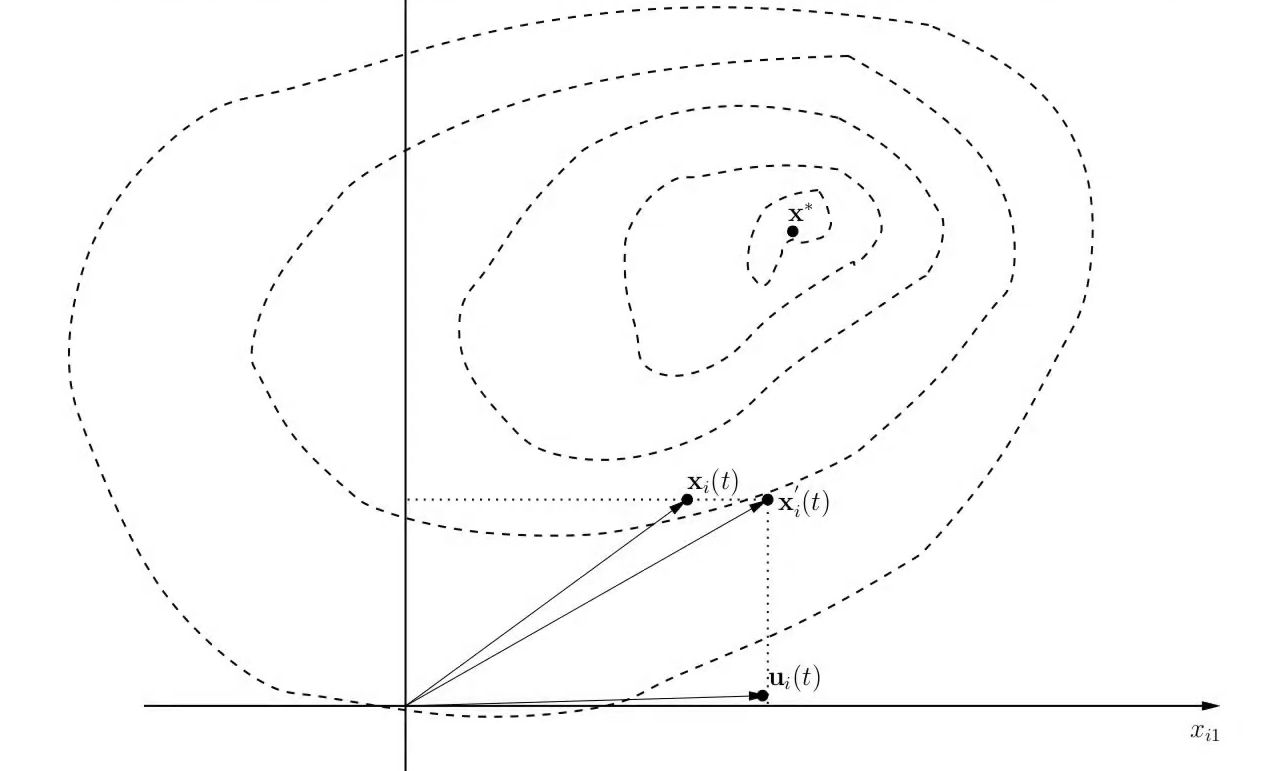
\includegraphics[width=1\textwidth]{imagenes/de-crossover.png}
    \end{center}
    \caption[Crossover en DE]{Esta figura ha sido seleccionada de \cite{10.5555/1557464}. Muestra de manera gráfica en un espacio bidimensional como funciona el operador de cruce al recombinar los genes/características de los vectores padre y ``trial''.}
\end{figure}

\subsubsection{Selección}
Si el vector hijo, al evaluarlo, tiene un valor \textbf{fitness} mejor que el vector padre, entonces se sustituye el vector $x_i$ por el vector $x^\prime_i$. De otra forma, el vector padre continuará en la población para la siguiente generación~\cite{storn_differential_1997}.

\section{Optimización por colonia de abejas artificial}
\subsection{Introducción}
El algoritmo del enjambre de abejas artificial es un algoritmo estocástico evolutivo, al igual que los ya mencionados anteriormente, que se basa en el comportamientos de los enjambres de abejas para la optimización de problemas. El modelo usado en este algoritmo depende de tres factores, las fuentes de alimento, las abejas buscadores empleadas y las abejas buscadoras desempleadas (hay dos tipos)~\cite{karaboga_idea_nodate}.

\subsection{Funcionamiento y Operadores}
Los operadores del algoritmo son los siguientes:
\begin{enumerate}
    \item \textbf{Abejas Empleadas (Employed Bees)}: Estas abejas están asociadas con fuentes de alimento específicas y son responsables de explotar estas fuentes. Llevan información sobre la fuente de alimento, incluyendo la distancia, la dirección y la rentabilidad, y comparten esta información dentro de la colmena, influyendo en las decisiones de otras abejas.

    \item \textbf{Abejas Observadoras (Onlooker Bees)}: Estas abejas esperan dentro de la colmena y toman decisiones sobre a qué fuentes de alimento dirigirse basándose en la información proporcionada por las abejas empleadas. Seleccionan las fuentes de alimento según la probabilidad que está directamente relacionada con la rentabilidad de las fuentes.

    \item \textbf{Abejas Exploradoras (Scout Bees)}: Son abejas que buscan nuevas fuentes de alimento sin información previa. Su rol es crucial para la exploración y el descubrimiento de nuevas fuentes de alimento. Cuando una fuente se agota o no mejora después de cierto número de intentos (determinado por un parámetro de control llamado "límite"), una abeja empleada puede convertirse en exploradora.
\end{enumerate}

Estos operadores trabajan en un ciclo repetitivo donde las abejas empleadas primero van a las fuentes de alimento y actualizan la información sobre su rentabilidad. Luego, las abejas observadoras seleccionan fuentes de alimento basadas en esta información actualizada y las abejas exploradoras buscan nuevas fuentes~\cite{karaboga_idea_nodate}. Este proceso se repite hasta cumplir con los criterios de terminación del algoritmo.

\section{Algoritmo de optimización del saltamontes}
\subsection{Introducción}
Los \textbf{grasshoppers} (saltamontes o langosta cuando están en enjambre) son insectos cuyo ciclo de vida consiste en tres etapas: \textit{huevo, ninfa, adulto}. Un saltamontes puede ser encontrado en el enjambre en su estado ninfa y adulto. La diferencia entre ninfa y adulto es la velocidad de movimiento con pasos pequeños en la ninfa y lo contrario en su vida adulta (Las soluciones adultas se encargan de la exploración y las ninfas de la explotación)~\cite{saremi_grasshopper_2017}.
\subsection{Funcionamiento y Operadores}
\subsubsection{Operador de posición (primera propuesta)}
La posición de un individuo se define en la siguiente ecuación:
\begin{equation}
    x_i = r_1s_1+r_2g_i+r_3a_i
\end{equation}
Donde $x_i$ es la posición del agente número $i$, $s$ la interacción social, $g$ la fuerza gravitacional, $a$ la advección del viento y $r_1, r_2, r_3$ son números aleatorios entre $[0,1]$.
Esta función de actualización de posición no puede ser usada para la optimización debido a que se alcanza la zona de comfort de manera prematura y no se converge en un punto específico~\cite{saremi_grasshopper_2017}.

\subsubsection{Posición (propuesta final)}

\begin{equation}
    X_i^d=c_1\left(\sum_{j=1,j\neq i}^N c_2\frac{ub_d-lb_d}{2}s(|x_j^d-x_i^d|)\frac{x_j-x_i}{d_{ij}}\right)+\hat{T_d}
    \label{eq:goa-position}
\end{equation}

Donde $ud_b$ es la cota superior en la dimensión $D$, $lb_d$ es la cota inferior en la dimensión $D$, $\hat{T_d}$ es el valor de la dimensión $D$ en el objetivo (la mejor solución encontrada hasta la fecha) y $c$ es el coeficiente decreciente para hacer cada vez más pequeña la zona de comfort, zona de atracción y zona de repulsión.

No se considera la gravedad (G) y la dirección del viento siempre es a favor del objetivo $\hat{T_d}$.

Una diferencia con otros algoritmos de enjambres como PSO es que \textbf{GAO} actualiza la posición de cada saltamontes a partir de la posición actual, el mejor punto encontrado hasta el momento y la posición de todos los otros agentes, mientras que \textbf{PSO} lo hace a partir de la posición actual del agente y la mejor posición encontrada~\cite{saremi_grasshopper_2017}.

Esto significa que PSO no tienen en cuenta al resto de agentes, mientras que GAO sí.

Los parámetros $c_1, c_2$ tienen dos propósitos:
\begin{itemize}
    \item $c_1$ $\rightarrow$ Reduce el movimiento del enjambre entero alrededor del objetivo, es decir, maneja la relación entre exploración y explotación para el conjunto global de soluciones.
    \item $c_2$ $rightarrow$ Reduce la zona de comfort y las regiones de repulsión y atracción. $s$ es la función que decide si un agente debe sentirse atraído o repelido al objetivo, mientras que $\frac{ub_d-lb_d}{2}$ decrece de manera lineal el espacio de búsqueda a medida que $c_2$ decrece.
\end{itemize}

Ha de tenerse en cuenta también que en el proceso de búsqueda, la exploración debe ir antes que la explotación. En los saltamontes sin embargo, la fase explotativa que es la \textbf{ninfa} es la que se da primero. Por ello el parámetro $c$ debe decrecer a medida que las iteraciones sobre el algoritmo van pasando. Este mecanismo hace que se promueva la explotación a medida que las iteraciones se incrementan, ya que se va reduciendo cada vez más el movimiento general del enjambre y se reduce la zona de comfort. $c$ se actualiza por tanto así:
\begin{equation}
    c = c_{\text{max}} - l \cdot \frac{c_{\text{max}} - c_{\text{min}}}{L}
\end{equation}

Donde $l$ es la iteración actual y $L$ el número máximo de iteraciones.

\begin{figure}[H]
    \begin{center}
        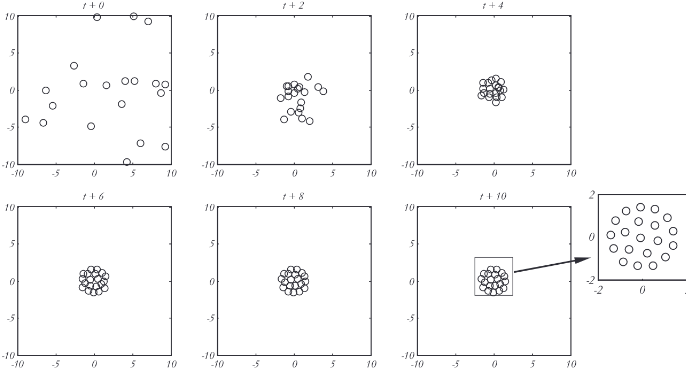
\includegraphics[width=0.8\textwidth]{imagenes/goa-position-convergence.png}
    \end{center}
    \caption[Convergencia en GOA]{Esta figura ha sido seleccionada de \cite{saremi_grasshopper_2017}. Muestra la convergencia de los ``saltamontes'' en tan solo unas pocas iteraciones usando la fórmula \ref{eq:goa-position}.}
\end{figure}

\section{Algoritmo de la libélula}
\subsection{Introducción}
Los \textbf{dragonflies} (libélulas en español) son pequeños insectos que se pueden ver en enjambre solo cuando cazan o migran, dando lugar a dos tipos de enjambre:
\begin{itemize}
    \item Las diferencias dadas entre ambos enjambres son notorias. En caza, se organizan en enjambres pequeños que vuelan en muchas direcciones en busca de comida. Este tipo de enjambre es llamado \textbf{estático}. Cuando se organizan en enjambres para migrar, estos son numerosos y vuelan en una sola dirección. Estos enjambres en contraposición a los anteriores son llamados \textbf{dinámicos}~\cite{mirjalili_dragonfly_2016}.
    \item Es obvio el paralelismo que se da entre las principales fases de la búsqueda optimizatoria (\textbf{exploración y explotación}). La fase dinámica es un paralelismo con la exploración, ya que se buscan pequeños objetivos en grupos por el espacio. La fase estática (explotación) se da cuando todos los agentes empiezan a migrar a una dirección concreta.
\end{itemize}


\subsection{Funcionamiento y Operadores}

\subsubsection{Separación}
\begin{equation}
    S_i = -\sum_{j=1}^N X - X_j
\end{equation}
Se refiere a la elusión estática de colisión entre individuos con su vecindario. Donde $X$ es la posición del agente actual y $X_j$ la posición de su vecino número $j$. Mientras que $N$ es el número total de agentes.

\subsubsection{Alineamiento}
\begin{equation}
    A_i = \frac{\sum_{j=1}^N V_i}{N}
\end{equation}
Se refiere a la coordinación de velocidad entre individuos de un vecindario. Donde $V_j$ es la velocidad del individuo número $j$ en el vecindario.

\subsubsection{Cohesión}
\begin{equation}
    C_i = \frac{\sum_{j=1}^N X_j}{N} - X
\end{equation}
Se refiere a la fuerza de atracción de los individuos hacia el centro de masa del vecindario. Se da por hecho un radio alrededor de cada libélula agrupando su vecindario, pues este es muy importante para el comportamiento de esta. En un enjambre dinámico, las libélulas tienden a alinear su vuelo al tiempo que mantienen una separación y cohesión adecuadas. En un enjambre estático, sin embargo, las alineaciones son muy bajas mientras que la cohesión es alta para atacar a las presas. Por lo tanto, se asigna a las libélulas pesos de alta alineación y baja cohesión cuando exploran el espacio de búsqueda y de baja alineación y alta cohesión cuando explotan el espacio de búsqueda. Para la transición entre exploración y explotación, los radios de vecindad se incrementan proporcionalmente al número de iteraciones~\cite{mirjalili_dragonfly_2016}.
\begin{figure}[H]
    \centering
    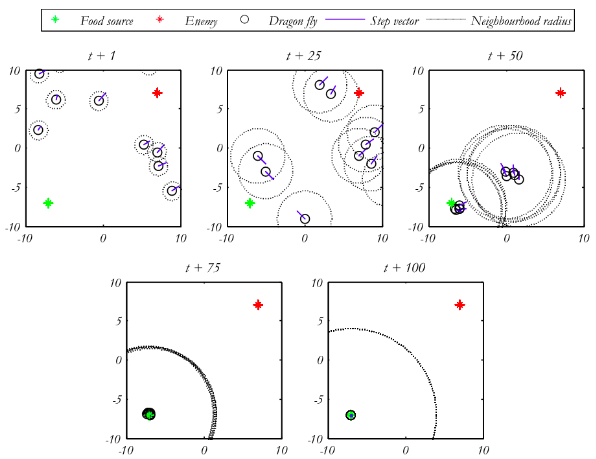
\includegraphics[width=0.9\textwidth]{imagenes/da-operators.png}
    \caption[Vecindario de libélulas]{Vecindario de libélulas~\cite{mirjalili_dragonfly_2016}.}
\end{figure}

\subsubsection{Atracción comida}
\begin{equation}
    F_i = X^+ - X
\end{equation}
La fuerza de atracción hacia la comida (la mejor posición encontrada hasta el momento). Donde $X^+$ es la mejor posición encontrada hasta el momento.

\subsubsection{Repulsión depredador}
\begin{equation}
    E_i = X^- + X
\end{equation}
La fuerza de repulsión hacia un depredador (la peor posición encontrada hasta el momento). Donde $X^-$ es la peor posición encontrada hasta el momento.

\subsubsection{Dirección}
\begin{equation}
    \Delta X_{t+1} = (sS_i + aA_i + cC_i + fF_i + eE_i) + w\Delta X_t
\end{equation}
El delta de $X$ indica el vector dirección del movimiento de las libélulas. Cada elemento en minúscula es el factor del operador al que multiplica, de forma que es posible acentuar el efecto de cada uno de estos con múltiples combinaciones.

\subsubsection{Posición}
\begin{equation}
    X_{t+1} = X_{t} + \Delta X_{t+1}
\end{equation}
El operador de actualización de posición.

\section{Algoritmo de optimización de ballenas}
\subsection{Introducción}
Simula el comportamiento de las ballenas jorobadas en la caza, utilizando tanto el azar como el mejor agente de búsqueda para perseguir a la presa. Además, emplea una espiral para simular el mecanismo de ataque de la red de burbujas de las ballenas jorobadas~\cite{mirjalili_whale_2016}.

\subsection{Funcionamiento y Operadores}
\subsubsection{Rodeado de presa}
\begin{equation}
    \vec{D}=|\vec{C}\cdot\vec{X}^*(t)-\vec{X}(t)|
\end{equation}
\begin{equation}
    \vec{X}(t+1)=\vec{X}^*(t)-\vec{A}\cdot\vec{D}
\end{equation}
Donde $t$ indica la iteración actual, $\vec{A}$ y $\vec{C}$ son vectores de coeficientes, $X^*$ es el vector de posición de la mejor solución encontrada hasta el momento y $\vec{X}$ es el vector posición.

Los vectores $\vec{A}$ y $\vec{C}$ se calculan como sigue:
\begin{equation}
    \vec{A}=2\vec{a}\cdot\vec{r}-\vec{a}
\end{equation}
\begin{equation}
    \vec{C}=2\cdot\vec{r}
\end{equation}
Donde $\vec{a}$ es decrementado linealmente desde $2$ hasta $0$ y $\vec{r}$ es un vector aleatorio con valores en $[0,1]$.

\subsubsection{Ataque de red de burbujas (explotación)}
\begin{itemize}
    \item \textbf{Mecanismo de encogimiento del cerco}
          Este mecanismo es conseguido mediante el decremento del valor de $\vec{a}$. El vector $\vec{A}$ es un vector de valores aleatorios en el intervalo $[-a,a]$ donde $a$ es decrementado desde $2$ hasta $0$.
          \begin{figure}[H]
              \centering
              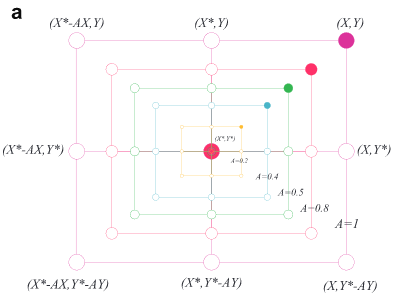
\includegraphics[width=0.5\textwidth]{imagenes/wao-shrinking-circle-prey-mechanism.png}
              \caption[Mecanismo de encogimiento del cerco]{Ataque de red de burbujas usando el mecanismo de encogimiento del cerco~\cite{mirjalili_whale_2016}.}
          \end{figure}

    \item \textbf{Mecanismo de actualización de posición en espiral}
          Este mecanismo calcula la distancia entre la ballena $(x,y)$ y la presa $(x^*, y^*)$. Una ecuación con forma de espiral es creada entonces entre la ballena y la presa para simular el comportamiento de estas al cazar.
          \begin{figure}[H]
              \centering
              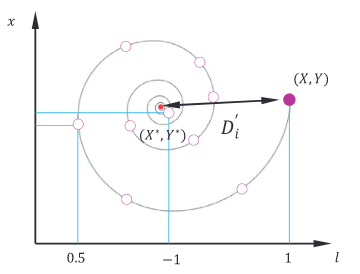
\includegraphics[width=0.5\textwidth]{imagenes/spiral-update-position-wao.png}
              \caption[Mecanismo de actualización de posición en espiral]{Ataque de red de burbujas usando el mecanismo de actualización de posición en espiral~\cite{mirjalili_whale_2016}.}
          \end{figure}

          \begin{equation}
              \vec{X}(t+1)=\vec{D}^{'}\cdot e^{bl}\cdot cos(2\pi l)+\vec{X}^*(t)
          \end{equation}
          Donde $\vec{D}^{'}=|\vec{X}^*(t)-\vec{X}(t)|$ e indica la distancia entre presa y ballena. $b$ es una constante para definir la forma de la espiral, $l$ es un número aleatorio entre $[-1,1]$.
\end{itemize}

Se utilizan ambos mecanismos, dependiendo de si cierto número $p$ aleatorio es mayor o menor a $0.5$.

\subsubsection{Búsqueda de la presa (exploración)}
El mismo método utilizando el vector $\vec{A}$ puede ser utilizado para la exploración. Se puede usar $\vec{A}$ con valores más grandes a $1$ o menores a $-1$ para forzar al agente a moverse lejos de otro agente.
\begin{equation}
    \vec{D}=|\vec{C}\cdot\vec{X}_{rand}-\vec{X}|
\end{equation}
\begin{equation}
    \vec{X}(t+1)=\vec{X}_{rand}-\vec{A}\cdot\vec{D}
\end{equation}
Cuando $|A|\geq 1$ $\rightarrow$ Exploración, cuando $|A|<1$ $\rightarrow$ Explotación.

\section{Algoritmo del murciélago}
\subsection{Introducción}
El algoritmo \textit{metaheurístico} de los murciélagos se basa en la capacidad de eco-localización de estos para detectar a su presa y cazarla finalmente. La eco-localización de los murciélagos no solo les permite detectar a su presa, sino discriminar entre distintos tipos de insectos. Más concretamente, este algoritmo se basa en los micro murciélagos, pues estos usan más frecuentemente la eco-localización en comparación a otras especies de murciélagos. Estos murciélagos emiten un pulso de sonido, el cual, rebota en los objetos y entidades cercanas, permitiendo al murciélago componer una ``visión'' general de sus alrededores. La frecuencia del pulso emitido podría estar relacionada con distintas estrategias de caza~\cite{yang_new_2010}.
\subsubsection{Acústica de la eco-localización}
Aunque cada pulso dura solo unos pocos milisegundos (entre 8 y 10 ms), mantiene una frecuencia constante, generalmente entre 25 kHz y 150 kHz. La longitud de onda ($\lambda$) de estos impulsos ultrasónicos, con una frecuencia ($f$) y velocidad del sonido ($v$) en el aire a 340 m/s, está dada por
\begin{equation}
    \lambda = \frac{v}{f}
\end{equation} 
con longitudes entre 2 mm y 14 mm para frecuencias de 25 kHz a 150 kHz, respectivamente. Esta longitud de onda coincide con el tamaño de las presas. Los murciélagos pueden detectar obstáculos tan pequeños como cabellos humanos, utilizando la eco-localización para construir un modelo 3D del entorno, y discriminando distancias, orientaciones y tipos de presas. Aunque los murciélagos tienen buena vista y olfato, utilizan principalmente la eco-localización para la detección de presas y la navegación eficiente~\cite{yang_new_2010}.

\subsection{Funcionamiento y Operadores}
Para simplificar:
\begin{itemize}
    \item Los murciélagos usan la ecolocación para percibir la distancia y distinguir alimento de barreras.
    \item Vuelan aleatoriamente con velocidad $v_i$ y frecuencia fija $f_{min}$, ajustando longitud de onda $\lambda$ y sonido $A_0$.
    \item Se asume que la intensidad del sonido varía desde $A_0$ hasta un mínimo $A_{min}$.
\end{itemize}

\end{document}
% %
%\input{capitulos/04_Materiales_y_Distorsiones}
% %
%\input{capitulos/05_Implementacion_y_Experimentos}
%
%\input{capitulos/06_Implementacion}
%
%\input{capitulos/07_Pruebas}
%
%\input{capitulos/06_Conclusiones}
%
%
\nocite{*}
% \bibliography{bibliografia/bibliografia}\addcontentsline{toc}{chapter}{Bibliografía}
% \bibliographystyle{unsrturl}
\newpage
\chapter{Bibliografía}
\printbibliography[heading=none, category=cited]

\thispagestyle{empty}
%%\input{apendices/paper/paper}
%\input{glosario/entradas_glosario}
% \addcontentsline{toc}{chapter}{Glosario}
% \printglossary
%\chapter*{}
%\thispagestyle{empty}
\end{document}